\FloatBarrier
\section{From Diagnosis to Candidate Interventions}
\label{sec:method}

The diagnosis specifies both \emph{what} fails (the quality of irreversible
commitments) and \emph{when} (when the committing frame is unreliable), and
makes a falsifiable prediction: interventions on image appearance or on
where-to-go should not move success, because the loss lives in the
reach-to-success conversion. To test this prediction we construct the most
natural candidate interventions the diagnosis suggests, spanning the pixel,
perception, and decision layers. A per-frame appearance oracle upper-bounds
per-frame arbitration over appearance. The instrument behind the test
(Figure~\ref{fig:pipeline}, Appendix) pairs the same frozen backbone on
clean and degraded versions of identical episodes.

\subsection{Per-Step Reliability Estimation}

We map each RGB frame to a scalar reliability $r\in[0,1]$ using a blind
detector bank that needs no reference frame or training. We combine cues
that respond to structure-preserving corruptions: mean luma for darkness,
global contrast and std.\ deviation for a haze veil, Laplacian energy for
blur, a dark-channel statistic for fog, and a noise estimate for sensor
noise. Each cue is calibrated once on a probe set so clean frames score
$r{\approx}1$ and corruptions lower $r$ monotonically
(Figure~\ref{fig:calibration}): clean $1.00$, low-light $0.65$,
motion-blur
$0.47$, fog $0.36$, Gaussian noise $0.20$. Throughout, $r$ serves as an
\emph{instrument}: it lets candidates gate on perceived trustworthiness,
but is not itself a contribution.

\begin{figure}[!t]
\centering
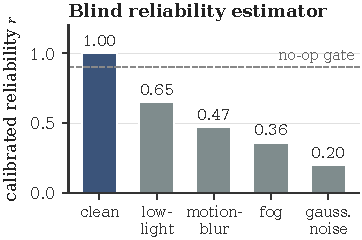
\includegraphics[width=0.52\columnwidth]{figures/fig_calibration.pdf}
\caption{\textbf{Blind reliability estimator $r$} on the calibration probe
set: clean frames score $r{\approx}1$; each structure-preserving
corruption lowers $r$ monotonically. Dashed line: the $r{=}0.9$ no-op
gate above which reliability-gated candidates reduce to the clean
baseline exactly.}
\label{fig:calibration}
\end{figure}

\subsection{Candidate 1 (Appearance): Blanket and Oracle-Gated Restoration}

The default remedy treats degradation as an image-quality problem and restores
the frame before the policy sees it. We include two variants. \emph{Blanket
restoration} (RES) always applies a low-light/denoising front-end. To upper-bound
\emph{any} test-time arbitration over appearance, we also define a \emph{per-frame
appearance oracle} (\textsc{OracleGate}) that, at every step, is allowed to pick
whichever of the degraded and restored views yields the better navigation
outcome. \textsc{OracleGate} is not deployable---it consults privileged
information---and it bounds any \emph{per-frame} router over restored
versus degraded appearance. If even \textsc{OracleGate} does not beat
blanket restoration, per-frame appearance arbitration has no headroom left
to exploit.

\subsection{Candidate 2 (Where-to-Go): Reliability-Gated Reweighting}

If appearance is not the lever, the diagnosis points to the decision layer.
A value-map navigator scores candidate headings by combining a
\emph{language--semantic term} $v_{\text{vlm+sem}}$ (which a corrupted frame
misleads) with a geometric frontier-coverage term $v_{\text{frontier}}$.
The reliability-gated reweighting candidate (R-Weight) takes a convex mixture
$v(a)=(1{-}\beta)v_{\text{vlm+sem}}(a)+\beta v_{\text{frontier}}(a)$, with
the mixing weight $\beta(r)$ gated by reliability: $\beta{=}0$ above
$\tau_{\text{gate}}{=}0.9$, and $\beta{=}\min(\beta_{\max},\alpha(1{-}r))$
below it ($\alpha{=}1$, $\beta_{\max}{=}0.6$), so on clean input R-Weight
reduces exactly to the backbone.

Together these candidates probe pixels (RES, OracleGate) and where-to-go
(R-Weight); \textsc{OracleGate} is an upper bound rather than a method, so
a collective failure to move success is a statement about \emph{where the
headroom is}, not about weak baselines. The Experiments section sweeps
four further families (commit timing/revocation, forced commitment,
temporal/multi-view aggregation, and a depth-based multimodal probe).
